\section{Objective}

Reference: \href{https://youtu.be/TkwXa7Cvfr8?si=V8cJG_DQAoA2fndE}{Watching Neural Networks Learn}

An \gls{AI_NN} is a \textit{non-linear mathematical tool} intended to simulate the human brain process by using simple units called artificial neurons arranged in structures known as layers.
\begin{center}
	An \gls{AI_NN} is a \textit{universal function approximator}. They are machines that create functions.
\end{center}

This non-linear mathematical tool can also be understood as a \textit{universal function approximator}. The \textit{Universal Approximation Theorem} states that \gls{AI_NN} with infinite neurons can approximate any function given the right weights. How to achieve this or how to come closer should be the objective of this segment. For example, the layer architecture, the activation function, and preparing the data are relevant topics to consider for finding the global minimum.

\paragraph{Different ways to look at it}
Many mathmatical field are in interplay when it comes to a \gls{AI_NN}.\\

Linear Algebra is mostly used when it comes to computing information though the network. Graph Theory can also be used to to the same thing, but is mostly considered when it comes to analyzing the structure of the neural network. 

\begin{description}
	\item[Linear Algebra] \glspl{AI_NN} can be represented using matrices and vectors, where each neuron's input and output can be described as linear combinations of the inputs with corresponding weights. Matrix operations such as multiplication, addition, and transposition are fundamental in understanding how information flows through the network during forward and backward propagation.
	\item[Graph Theory] \glspl{AI_NN} can be represented as directed graphs, where neurons correspond to nodes and connections between neurons correspond to edges. Graph theory concepts are useful for analyzing the structure of neural networks, including connectivity patterns and network architectures.
\end{description}

Given a certain structure of the network \textit{optimisation} with main tool from \textit{calculus}: \textit{gradient descent} is used to find the parameter that reduces the loss function.\footnote{
	While calculus and optimization are related and often used together in the context of machine learning and neural networks, they are distinct mathematical concepts with different focuses.
}

\begin{description}
	\item[Optimization] \gls{AI_NN} are trained by optimizing a loss function with respect to the network's parameters. Optimization theory provides a framework for selecting appropriate optimization algorithms, tuning hyperparameters, and understanding convergence properties. While calculus provides the mathematical framework for computing gradients and understanding the behavior of optimization algorithms, optimization theory encompasses a wider range of techniques beyond calculus, such as convex optimization, linear programming, and heuristic algorithms.
	\item[Calculus (Optimization)] Calculus is essential for optimizing the parameters (weights and biases) of \gls{AI_NN} through techniques like gradient descent and its variants. Understanding derivatives is crucial for computing gradients, which indicate how the loss function changes with respect to changes in the network's parameters. Calculus helps in finding the direction and rate of change that minimizes or maximizes a function, which is crucial for training neural networks to minimize the loss function.
\end{description}

The field of \textit{probability and statistics} as well as \textit{information theory} are used for multiple aspects of \glspl{AI_NN}. For example the former can be used to preparing or preprocessing of data, model evaluation and bringing into context the uncertainty in predictions. The later will also be used for finding the features in the dataset as well as analysing the information flow inside a \gls{AI_NN}.

\begin{description}
	\item[Probability and Statistics] ANNs can be viewed as probabilistic models, especially in the context of Bayesian neural networks, where uncertainty is explicitly modeled. Statistical techniques are used for data preprocessing, model evaluation, and uncertainty estimation in predictions.
	\item[Information Theory] Information theory concepts, such as entropy and mutual information, can be used to analyze the information flow within neural networks. Compression techniques inspired by information theory, such as autoencoders, are used for feature extraction and dimensionality reduction.
\end{description}

The field of \textit{functional analysis} provides the tools to analyze the natrue of the universal function approximator, called \gls{AI_NN}.

\begin{description}
	\item[Functional Analysis] \glspl{AI_NN} can be viewed as function approximators, and functional analysis provides tools for analyzing the properties of these approximations. Understanding function spaces and convergence properties is relevant when studying the expressive power and generalization abilities of neural networks. 
\end{description}

\begin{sidewaystable}[h] %!ht
	\centering
	\begin{tabular}{|p{3cm}|*{6}{p{3cm}|}}
		\hline
		\textbf{Mathematical Fields} & \textbf{Featurization} & \textbf{Data Processing} & \textbf{Model Architecture} & \textbf{Optimization Parameter} & \textbf{Evaluation} & \textbf{General Assessment} \\ \hline
		\textbf{Linear Algebra} & ~ & ~ & ANN represented as matrices and vectors; Input and Output linear combination & ~ & ~ & ~ \\ \hline
		\textbf{Graph Theory} & ~ & ~ & ANN represented as directed graphs; Analyzing the structure of the network & ~ & ~ & ~ \\ \hline
		\textbf{Information Theory} & Compression techniques: autoencoder; dimensionality reduction & ~ & ~ & ~ & ~ & ~ \\ \hline
		\textbf{Optimization (e.g., Calculus)} & ~ & ~ & ~ & Techniques like gradient descent and weights and biases & ~ & ~ \\ \hline
		\textbf{Probability Theory (Stochastic)} & ~ & Techniques for data processing steps & In case of a BNN & ~ & Model evaluation; uncertainty estimation in predictions & ~ \\ \hline
		\textbf{Functional Analysis} & ~ & ~ & ~ & ~ & ~ & Understanding the expressive power/general ability \\ \hline
	\end{tabular}
	\caption{Workflow Diagram of Mathematical Perspectives in ANN}
\end{sidewaystable}

\paragraph{Landscape of different Architectures}

There are different kinds of \gls{AI_NN}, for example: convolutional, recursive. This segment will focus on \textit{feed-forward} networks. A Feed-Forward is usually a non-linear regression or classification with a sigmoidal activation and a multilayer perceptron.

\begin{figure}[H]
	\centering
	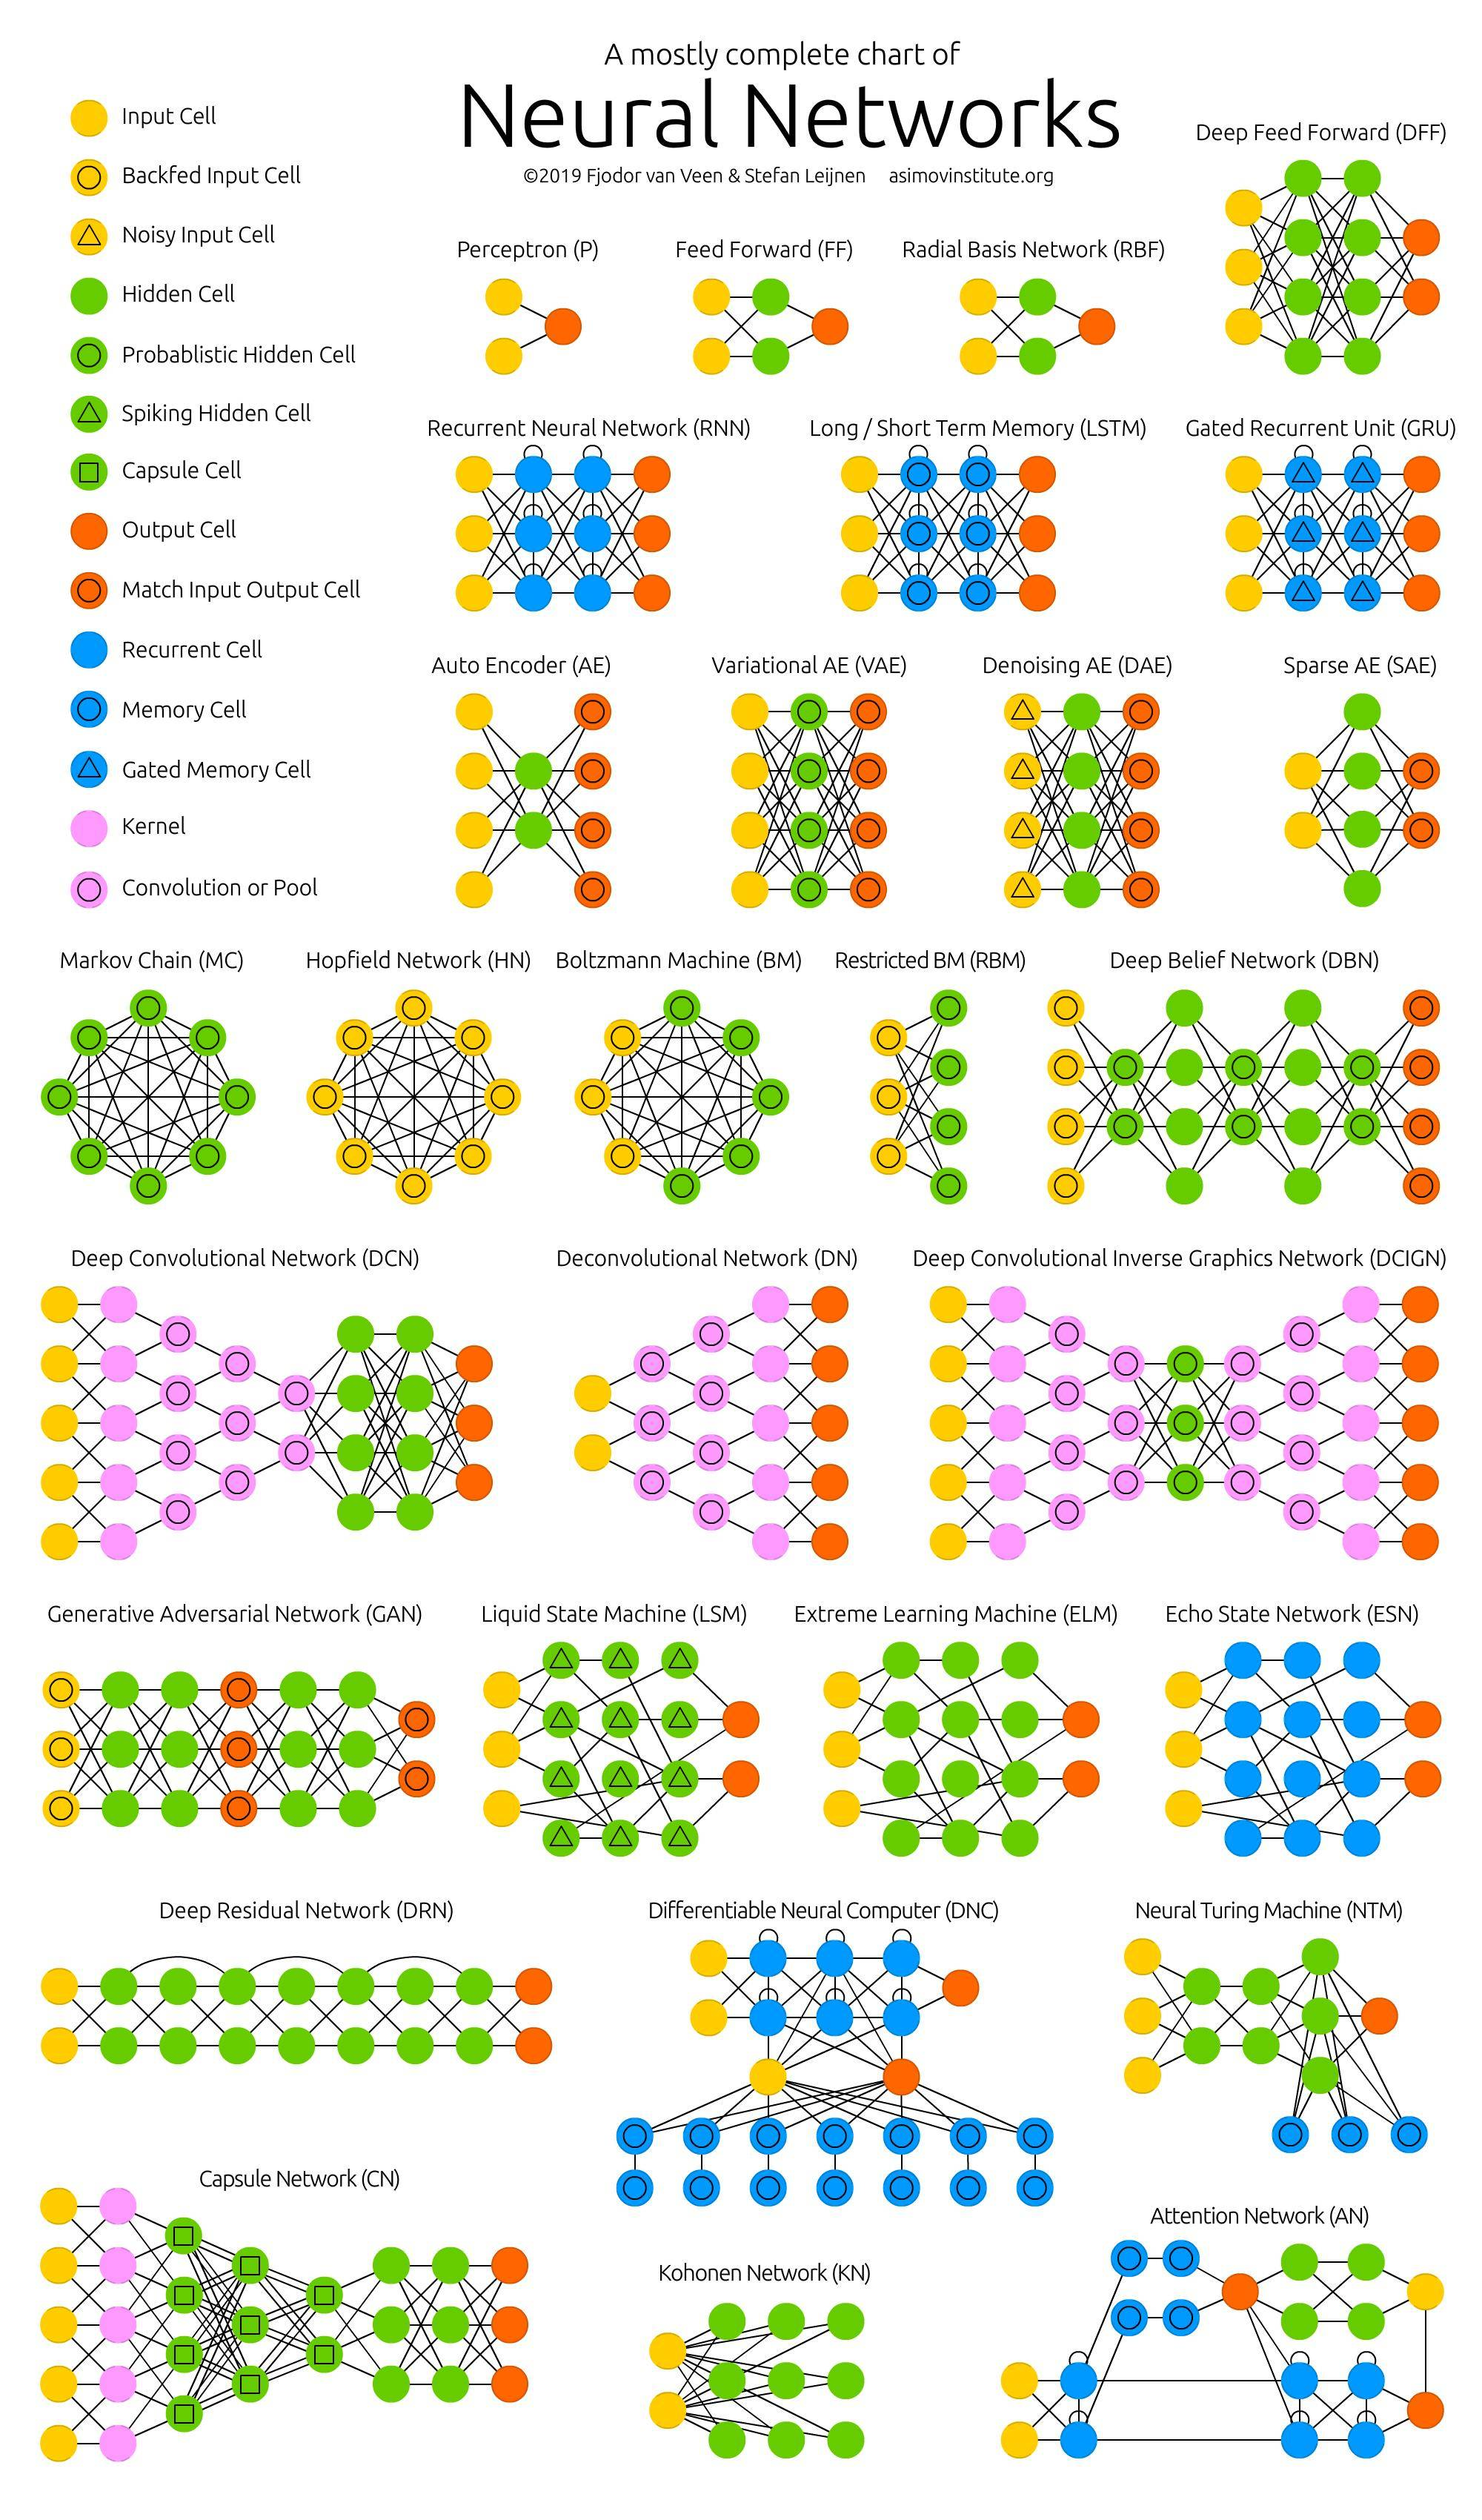
\includegraphics[scale = 0.1]{attachment/chapter_AML/Scc035}
	\caption{Types of artificial neural networks.}
\end{figure}

\section{Multilayer Perceptrons (MLP)}

\paragraph{Mathematical Foundations}
Reference, siehe auskommentierte Link und dem Buch \cite{MLK_Andr_Buk}[93] % \href{https://www.mdpi.com/2075-1680/11/2/80#:~:text=Hence%2C%20each%20artificial%20neuron%20may,b%20)%20%2C%20see%20Figure%201.}{https://www.mdpi.com/2075-1680/11/2/80#:~:text=Hence%2C%20each%20artificial%20neuron%20may,b%20)%20%2C%20see%20Figure%201.}
\begin{description}
	\item \gls{AI_NN}: Nonlinear Mathematical Tools as Universal Function Approximators
	\item Each node combines an \textit{affine linear function} and a nonlinear \textit{activation function}. 
\end{description}

\glspl{AI_NN} are nonlinear mathematical tools\footnote{However, there is a possibility to design it so that it can be a linear function.}, intended to mimic human brain processes by stacking simple neurons together. The simplest unit of an \gls{AI_NN} is called a \textit{Neuron}. They are structured in \textit{layers}. The learning process for humans is called training, while for \glspl{AI_NN} it is referred to as training.

A layer can be represented as a \textit{parameterized function}. From the perspective of a directed graph, each node can be represented as an \textit{affine linear function}. The combination of each layer can be understood as a new \textit{affine linear function} [for a given neuron].

The nonlinear quality of an \gls{AI_NN} arises from the \textit{activation function}.

\paragraph{Transformer Function} Given the input $x^t$\footnote{
	The initial input of the layer can be understood as \textit{features}, which can be represented as a vector  $x^t = (x_1, \dots, x_n)$
}. These are processed in a \textit{neuron} through \textit{weights} $w_i, i=1,\dots, n$, producing $z$, which then produces the final output $y$ through some function $\phi$, $\phi(z) = y$.

The output $z$ is the result of processing the $n-x_i$ weightily:
\begin{align}
z &= (w_1, \dots, w_n) \left(\begin{matrix}
		x_1 \\
		\vdots \\
		x_n
	\end{matrix} \right) + b \\
  &= \sum_{i=1}^n x_i\cdot w_i +b = w^t x + b,
\end{align}
where $b$ is called \textit{bias}. This should give the system more flexibility by imitating a human filter. This \textit{affine function} can be changed into a linear function, where $b$ is set as $w_0$ and $x_0 = 1$:
\begin{align}
z &= (w_0, \dots, w_n) \left(\begin{matrix}
		x_0 = 1 \\
		\vdots \\
		x_n
	\end{matrix} \right) \\
  &= \sum_{i=0}^n x_i\cdot w_i = w^t x.
\end{align}
To avoid the notation of the transpose, it can be represented by $w\cdot x$.

However, depending on the needs, these processes can be viewed as affine or linear functions. In either case, processing the input $x_i$ resulting in $z$ is called a \textbf{transfer function}. Depending on the needs different transformers can be used. The most popular or most used is the sum operator $\sum$:

\begin{figure}[h]
\centering
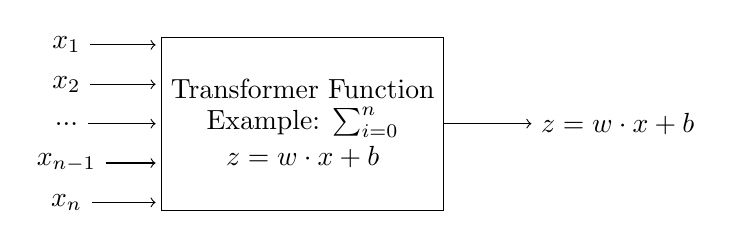
\begin{tikzpicture}
    % Nodes
    \foreach \x/\name in {1/x_1, 2/x_2, 3/. .. , 4/x_{n-1}, 5/x_n}
        \node at (0,-\x*0.5) (x\x) {$\name$};
  
    
    %% Node (e.g. Boxes, Symboles)    
    % Transformer Box
     \node[draw, minimum width=2cm, minimum height= 2.2 cm] at (3,-1.5) (transformer) {\shortstack{Transformer Function\\ Example: $\sum_{i=0}^n $\\ $z = w\cdot x + b$}};
    
    
    % Output activation symbole
    \node[right of=transformer, node distance=4cm] (z) {$z = w\cdot x + b$};
    
    
    %% Arrows
    % *0.5 reduces the distance
    \foreach \x in {1,2,...,5}*0.5
        \draw[->] (x\x.east) -- ([xshift=-2pt]transformer.west |- x\x);
    \draw[->] (transformer.east) -- (z.west);

    
\end{tikzpicture}
\caption{One perceptron, aka neuron}
\end{figure}

\paragraph{Activation Function}
The function $y=\phi(z)$ is known as the \textit{activation function} and it is this function that is resonsible for the non-linearity of the process. The function can be $"$freely$"$ selected, if it is fullyfilling certain criteria. \\

Each neuron can be regared as a mathematical function that is changing the \textit{transformation function} and the \textit{activation} with the inputs togehter: $y=\phi(z)= \phi\left(wx+b\right)$:

\begin{figure}[h]
\centering
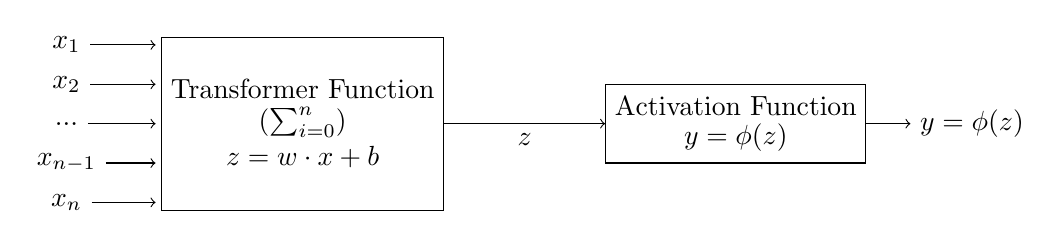
\begin{tikzpicture}
    % Nodes
    \foreach \x/\name in {1/x_1, 2/x_2, 3/. .. , 4/x_{n-1}, 5/x_n}
        \node at (0,-\x*0.5) (x\x) {$\name$};
  
    
    %% Node (e.g. Boxes, Symboles)
	 % Activation Box
    \node[draw, minimum width=2cm, minimum height= 1 cm] at (8.5,-1.5) (activation) {\shortstack{Activation Function \\ $y = \phi(z)$}};
    
    % Transformer Box
     \node[draw, minimum width=2cm, minimum height= 2.2 cm] at (3,-1.5) (transformer) {\shortstack{Transformer Function\\  $\left(\sum_{i=0}^n \right)$\\ $z = w\cdot x + b$}};
    
    
    % Output activation symbole
    \node[right of=activation, node distance=3cm] (phi) {$y = \phi(z) $};
    
    
    %% Arrows
    % *0.5 reduces the distance
    \foreach \x in {1,2,...,5}*0.5
        \draw[->] (x\x.east) -- ([xshift=-2pt]transformer.west |- x\x);
    \draw[->] (transformer.east) -- node[below] {$z$}(activation.west);
    \draw[->] (activation.east) -- (phi.west);

    
\end{tikzpicture}
\caption{One perceptron, aka neuron}
\end{figure}

\pagebreak
\paragraph{Feed-Forward}

As discussed before, the entirety of \glspl{AI_NN} can be understood as mathematical functions with an input $x$ and an output $y$.

\begin{align}
	f_{NN}(x) = y
\end{align} 

To combine each neuron, the output of each neuron is sent to all neurons in the next layer. This forwarding of information is called \textit{feed-forward}. From the perspective of a function, this is called \textit{verschachteln}. Each neuron in each layer (hidden layer) receives the output of the previous neurons. This neuron is then called a \gls{MLP}.

\begin{Definition}{Multilayer Perceptron}
	
	A \gls{MLP} is a function $f_l:\R^n \rightarrow \R$. It is called an $n-L-m$ perceptron, with $n$ inputs, $L$ hidden layers, and $m$ outputs.
	
	\begin{align}
		y = f^{(l)}(\vec{x}) = f_{l-1}\left(f_{l-2}\left(...\left(f_{0}(\vec{x})\right)\right)\right).
	\end{align}
	
	Where $f^{(i)}(\vec{z}) \stackrel{def}{=} \phi_l\left( \Matrix[W]^{(l)}\vec{z} + b^{(l)}\right)$.
\end{Definition}


\begin{figure}[h]
	\centering
\scalebox{0.6}{%
	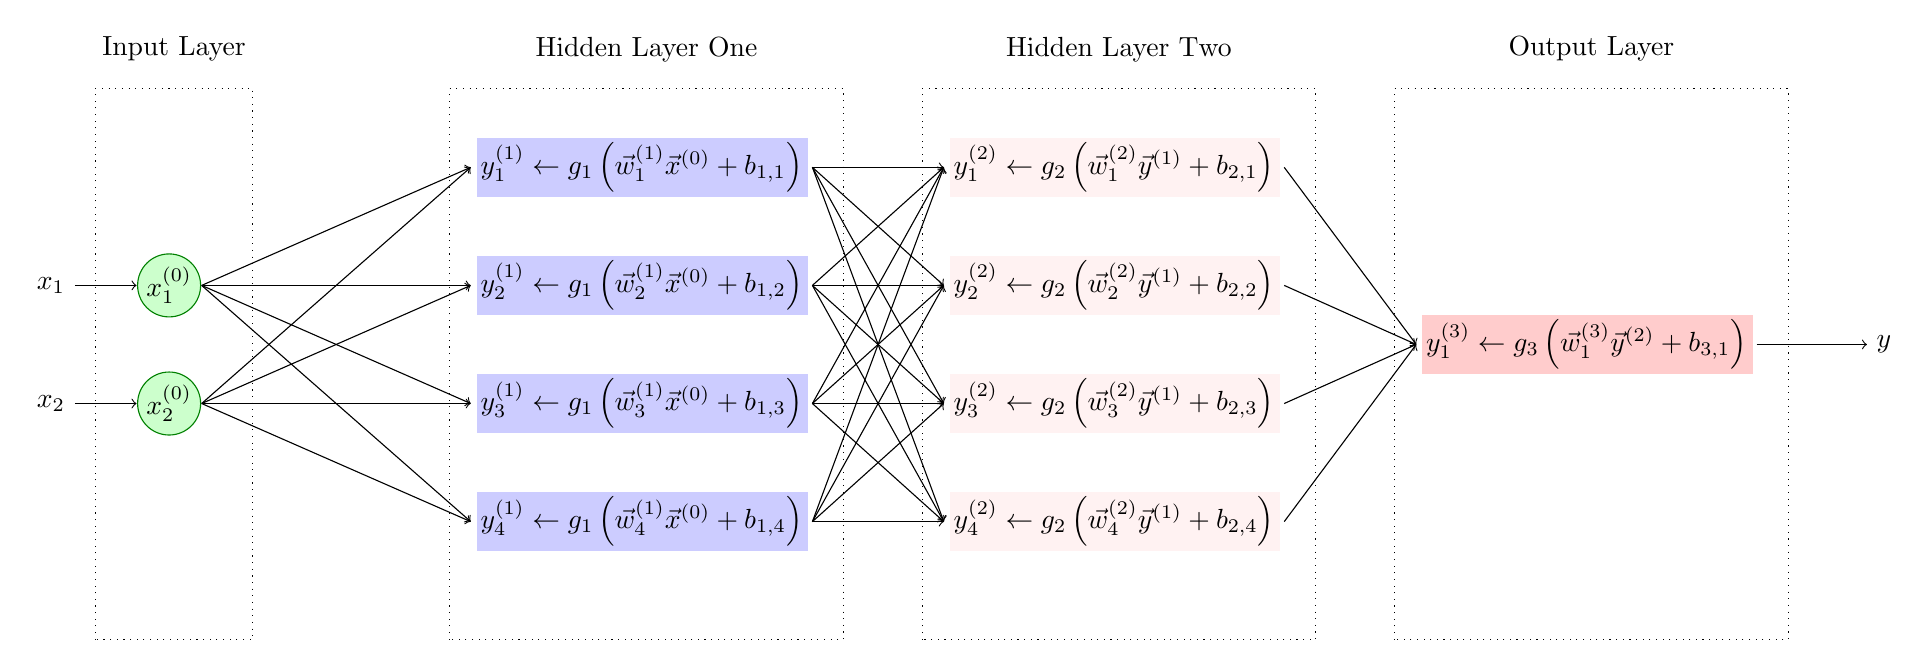
\begin{tikzpicture}
		
		% Drawing input on the left side each input layer
		\def\movefactorZeroZeroCircles{-7.5}
		\foreach \x/\layerindex in {1/x}{
			\foreach \y/\neuroindex in {6/1,4/2}{
				\node[name=\layerindex_\neuroindex] at (\x*3.25 +\movefactorZeroZeroCircles -0.8125,\y*0.75) {% function desciption
					$x_\neuroindex$
				};
				
			}
		}
		
		% Input layer with two neurons
		\draw[dotted] (-4.5,0) rectangle ++(2,7);
		\node at (-3.5,7.5) {Input Layer}; % Label for the Hidden layer one
		
		% Drawing circles on the left side of the Hidden layer one
		\def\movefactorZeroCircles{-6}
		\foreach \x/\layerindex in {1/0}{
			\foreach \y/\neuroindex in {6/1,4/2}{
				\filldraw[fill=green!20, draw=green!50!black] (\x*3.25 +\movefactorZeroCircles -0.8125,\y*0.75) circle circle (0.4);
				\node[name=\layerindex_\neuroindex] at (\x*3.25 +\movefactorZeroCircles -0.8125,\y*0.75) {% function desciption
					$x^{(\layerindex)}_{\neuroindex}$
				};
			}
		}   
		
		% Hidden layer one with four neurons
		\draw[dotted] (0,0) rectangle ++(5,7);
		\node at (2.5,7.5) {Hidden Layer One}; % Label for the Hidden layer one
		
		% Drawing neurons and displaying function in the Hidden layer one
		\foreach \x/\layerindex in {1/1}{
			\def\forwardedlayerindex{0}
			\foreach \y/\neuroindex in {8/1,6/2,4/3,2/4}{
				\fill[blue!20] (\x*3.25 -2.9,\y*0.75-0.375) rectangle ++(4.2,0.75);
				\node[name=\layerindex_\neuroindex] at (\x*3.25-0.8125,\y*0.75-0.375+0.375) {% function desciption
					$y_\neuroindex^{(\layerindex)} \leftarrow g_\layerindex \left(\vec{w}^{(\layerindex)}_{\neuroindex}\vec{x}^{(\forwardedlayerindex)}+b_{\layerindex,\neuroindex}\right)$
				};
			}
		}
		
		% Second box with four neurons
		\draw[dotted] (6,0) rectangle ++(5,7);
		\node at (8.5,7.5) {Hidden Layer Two}; % Label for the second box
		
		% Drawing neurons and displaying function in the second box
		\def\movefactorSecondBox{6}
		\def\forwardedlayerindex{1}
		\foreach \x/\layerindex in {1/2}{
			\foreach \y/\neuroindex in {8/1,6/2,4/3,2/4}{
				\fill[pink!20] (\x*3.25 + \movefactorSecondBox -2.9,\y*0.75-0.375) rectangle ++(4.2,0.75);
				\node[name=\layerindex_\neuroindex] at (\x*3.25+ \movefactorSecondBox -0.8125,\y*0.75-0.375+0.375) {% function desciption
					$y_\neuroindex^{(\layerindex)} \leftarrow g_\layerindex \left(\vec{w}^{(\layerindex)}_{\neuroindex}\vec{y}^{(\forwardedlayerindex)}+b_{\layerindex,\neuroindex}\right)$
				};
			}
		}
		
		% Third box with a single inner box
		\draw[dotted] (12,0) rectangle ++(5,7);
		\node at (14.5,7.5) {Output Layer}; % Label for the third box
		
		% Drawing neurons and displaying function in the third box
		\def\movefactorThirdBox{6}
		\def\forwardedlayerindex{2}
		\foreach \x/\layerindex in {1/3}{
			\foreach \y/\neuroindex in {5/1}{
				\fill[red!20] (\x*3.25 + \movefactorSecondBox + \movefactorThirdBox -2.9,\y*0.75-0.375) rectangle ++(4.2,0.75);
				\node[name=\layerindex_\neuroindex] at (\x*3.25+ \movefactorSecondBox + \movefactorThirdBox -0.8125,\y*0.75-0.375+0.375) {% function desciption
					$y_\neuroindex^{(\layerindex)} \leftarrow g_\layerindex \left(\vec{w}^{(\layerindex)}_{\neuroindex}\vec{y}^{(\forwardedlayerindex)}+b_{\layerindex,\neuroindex}\right)$
				};
			}
		}
		
		% Arrows connecting right side of input to left side of the corresponding cicle
		\draw[->] (x_1) -- (0_1);
		\draw[->] (x_2) -- (0_2);
		
		% Arrows connecting right side of circels to left side of the corresponding inner box of the Hidden layer one
		\foreach \x in {1,2}
		\foreach \y in {1,2,3,4}
		\draw[->] (0_\x.east) -- (1_\y.west);
		
		
		% Arrows connecting right side of neurons of the Hidden layer one to left side of the corresponding inner box of the second box
		\foreach \x in {1,2,3,4}
		\foreach \y in {1,2,3,4}
		\draw[->] (1_\x.east) -- (2_\y.west);
		
		% Arrows connecting right side of neurons of the second box to left side of the single inner box of the third box
		\foreach \x in {1,2,3,4}
		\foreach \y in {1}
		\draw[->] (2_\x.east) -- (3_\y.west);
		
		% Arrow from right side of inner box of the third box to slightly outside the dotted line with label y on the right hand side
		\draw[->] (3_1.east) -- (6+\movefactorSecondBox+\movefactorThirdBox,5*0.75) node[right] {$y$};
		
		
		
	\end{tikzpicture}
}
\caption{\gls{MLP} with two hidden layer, one input vector and one output layer}
\end{figure}


In this example, the output of the \gls{MLP} $y^{(1)}_1$ is calculated by the activation function $g_1$ for the hidden layer $1$. The weight vector $\vec{w}^{(0)}_1$ has dimension $2$, as it receives two inputs $x^{(1)}_1$ and $x^{(1)}_2$, along with the scalar bias $b^{(1)}_1$. In the next layer, the dimension of each weight vector is $4$, as each \gls{MLP} receives inputs $y^{(1)}_1$, $y^{(1)}_2$, $y^{(1)}_3$, and $y^{(1)}_4$ from the previous layer.

